\documentclass[12pt]{amsart}

%%%%%%%%%%%%%%%%%%%%%%%%%%%%%%%%%%%%%%%%%%%%%%%%
% Core Math Packages
%%%%%%%%%%%%%%%%%%%%%%%%%%%%%%%%%%%%%%%%%%%%%%%%
\usepackage{mathrsfs}     % Script fonts
\usepackage{bm}           % Bold math symbols
\usepackage{esvect}       % Vector arrows: \vv


%%%%%%%%%%%%%%%%%%%%%%%%%%%%%%%%%%%%%%%%%%%%%%%%
% Cross-referencing Packages and Label Customization
%%%%%%%%%%%%%%%%%%%%%%%%%%%%%%%%%%%%%%%%%%%%%%%%
\usepackage[colorlinks=true, linkcolor=MidnightBlue, citecolor=OliveGreen, urlcolor=RoyalBlue]{hyperref}  % Hyperlinks in PDF
\usepackage[nameinlink,capitalize]{cleveref}  % Smart cross-references with label names
\crefname{figure}{Figure}{Figures} % prevents cleveref from abbreviating
\Crefname{figure}{Figure}{Figures} % prevents cleveref from abbreviating
\crefname{table}{Table}{Tables} % prevents cleveref from abbreviating
\Crefname{table}{Table}{Tables} % prevents cleveref from abbreviating
\crefname{equation}{Equation}{Equations} % prevents cleveref from abbreviating
\Crefname{equation}{Equation}{Equations} % prevents cleveref from abbreviating
\crefname{page}{page}{pages} % lowercase for \cref and \cpageref

%%%%%%%%%%%%%%%%%%%%%%%%%%%%%%%%%%%%%%%%%%%%%%%%
% Utility and Layout Packages
%%%%%%%%%%%%%%%%%%%%%%%%%%%%%%%%%%%%%%%%%%%%%%%%
\usepackage[margin=1.25in]{geometry}
\usepackage{booktabs}  % Better horizontal rules
\usepackage{array}     % Column alignment customization
\usepackage[usenames,dvipsnames,table,xcdraw]{xcolor}  % Enhanced color names
\usepackage{graphicx}     % Image inclusion
\usepackage{multicol}     % Multiple column environments
\usepackage{enumitem}     % Customizable lists
\usepackage{todonotes}    % TODOs and margin notes
\usepackage{accents}      % For accents like \uvec
\usepackage[backend=biber,style=authoryear-comp]{biblatex}
\addbibresource{refs.bib}


%%%%%%%%%%%%%%%%%%%%%%%%%%%%%%%%%%%%%%%%%%%%%%%%
% TikZ and PGFPlots (Optional)
%%%%%%%%%%%%%%%%%%%%%%%%%%%%%%%%%%%%%%%%%%%%%%%%
\usepackage{tikz}
\usepackage{pgfplots}
\pgfplotsset{compat=1.9}
\usetikzlibrary{
  arrows.meta,
  angles,
  quotes,
  shapes,
  positioning,
  decorations.markings,
  shadings
}
\usepgfplotslibrary{fillbetween, colormaps, external}


%%%%%%%%%%%%%%%%%%%%%%%%%%%%%%%%%%%%%%%%%%%%%%%%
% Custom Commands
%%%%%%%%%%%%%%%%%%%%%%%%%%%%%%%%%%%%%%%%%%%%%%%%

%%%% Math Sets and Common Symbols %%%%
\newcommand{\R}{\mathbb{R}}
\newcommand{\Q}{\mathbb{Q}}
\newcommand{\Z}{\mathbb{Z}}
\newcommand{\N}{\mathbb{N}}
\newcommand{\C}{\mathbb{C}}
\newcommand{\ep}{\varepsilon}
\newcommand{\grad}{\nabla}

%%%% Math Operators %%%%
\DeclareMathOperator{\Int}{int}
\DeclareMathOperator{\proj}{proj}
\DeclareMathOperator{\orth}{orth}
\DeclareMathOperator{\comp}{comp}
\DeclareMathOperator{\sgn}{sgn}

%%%% Calligraphic Symbols %%%%
\newcommand{\p}{\mathcal{P}}
\newcommand{\T}{\mathcal{T}}
\newcommand{\Line}{\mathcal{L}}

%%%% Vectors and Bold Symbols %%%%
\newcommand{\bvec}[1]{\vv{\mathbf{#1}}}
\newcommand{\uvec}[1]{\boldsymbol{\hat{\textbf{#1}}}}
\newcommand{\uveci}{\uvec{\i}}
\newcommand{\uvecj}{\uvec{\j}}
\newcommand{\uveck}{\uvec{k}}

%%%% Annotation / Notes %%%%
\newcommand{\note}[2][]{\todo[caption={#2}, color=white,size=\footnotesize,noline,#1]{\renewcommand{\baselinestretch}{1}\selectfont#2\par}}

%%%% Improved Dot Product %%%%
\makeatletter
\newcommand*{\dotprod}{}% Check if undefined
\DeclareRobustCommand*{\dotprod}{%
  \mathbin{\mathpalette\dotprod@{}}%
}
\newcommand*{\dotprod@scalefactor}{.6}
\newcommand*{\dotprod@widthfactor}{1.15}
\newcommand*{\dotprod@}[2]{%
  \sbox0{$#1\vcenter{}$}%
  \sbox2{$#1\cdot\m@th$}%
  \hbox to \dotprod@widthfactor\wd2{%
    \hfil
    \raise\ht0\hbox{%
      \scalebox{\dotprod@scalefactor}{%
        \lower\ht0\hbox{$#1\bullet\m@th$}%
      }%
    }%
    \hfil
  }%
}
\makeatother


%%%%%%%%%%%%%%%%%%%%%%%%%%%%%%%%%%%%%%%%%%%%%%%%
% Theorem Environments
%%%%%%%%%%%%%%%%%%%%%%%%%%%%%%%%%%%%%%%%%%%%%%%%
\theoremstyle{plain} 
\newtheorem{theorem}{Theorem}
\newtheorem{proposition}[theorem]{Proposition} 
\newtheorem{corollary}[theorem]{Corollary} 
\newtheorem{conjecture}[theorem]{Conjecture} 
\newtheorem{lemma}[theorem]{Lemma}

\theoremstyle{definition} 
\newtheorem{definition}[theorem]{Definition}
\newtheorem{example}[theorem]{Example}
\newtheorem{exercise}[theorem]{Exercise}
\newtheorem{remark}[theorem]{Remark}
\newtheorem{problem}[theorem]{Problem}


%%%%%%%%%%%%%%%%%%%%%%%%%%%%%%%%%%%%%%%%%%%%%%%%
% Beginning of the Document
%%%%%%%%%%%%%%%%%%%%%%%%%%%%%%%%%%%%%%%%%%%%%%%%
\begin{document}

\title{Sample \LaTeX\  document}

\author{Isaac Newton} \address{Dickinson College\\ Carlisle, PA 17013}\email{newtoni@dickinson.edu}


\date{\today}
\begin{abstract}
This is where you will write your abstract, containing a brief description of all of your brilliant mathematical results.
\end{abstract}

\maketitle
\section{Introduction}\label{sec:intro}
Put       your          introduction        here.

% Notice that vertical extra space doesn't show up in the final product

\section{Main results}\label{sec:main}

You can create mathematics inline such as $\frac{a}{b}$ or $\lim_{x\to 0}\frac{\sin x}{x}=1$ or $\displaystyle\lim_{x\to 0}\frac{\sin x}{x}=1$. You can also put the mathematics on its own line, \[\sum_{k=0}^\infty \frac{1}{2^k}=2.\]


We can write in \emph{italics} and \textbf{boldface}. We can also \underline{underline text}. We can make ``blackboard bold'' letters (notice how we made the quotes) to denote the natural numbers, rational numbers, real numbers, and integers.

\[\mathbb{Q}=\left\{\frac{a}{b}\in\mathbb{R}:a,b\in\mathbb{Z},\ b\ne 0\right\}\]

We can make matrices of various types.

\[A=\left(\begin{array}{cccc}
1 &0 &4 &-1\\
0 &1 &-3 &1 \\
0 &0 &0 &1
\end{array}\right)=
\left[\begin{array}{cccc}
1 &0 &4 &-1\\
0 &1 &-3 &1 \\
0 &0 &0 &1
\end{array}\right]\]




We can make unordered lists.

\begin{itemize}
\item
Alabama
\item
Alaska
\begin{itemize}
\item
Juno
\item
Fairbanks
\item
Anchorage
\end{itemize}
\item
Arizona
\end{itemize}

We can also make ordered lists.

\begin{enumerate}
\item
Cat
\item
Dog
\begin{enumerate}
\item
Golden retriever
\item
Black lab
\item
Mutt
\end{enumerate}
\item
Gerbil
\item
Hamster
\end{enumerate}


LaTeX will format definitions, theorems, corollaries, propositions, lemmas, etc. For instance, we have the following examples.

\begin{definition}[Definition of limit]\label{def:limit}
Let $f$ be a function defined on an open interval containing $x=a$, but perhaps not at $x=a$. We say $\displaystyle\lim_{x\to a}f(x)=L$ if for any $\epsilon>0$ there exists $\delta>0$ such that $|f(x)-L|<\epsilon$ whenever $0<|x-a|<\delta$.
\end{definition}

\begin{definition}\label{def:deriv}
The \emph{ derivative} of $f$ is defined to be $\displaystyle f^\prime(x)=\lim_{h\to 0}\frac{f(x+h)-f(x)}{h}$, if this limit exists.
\end{definition}
 
\begin{theorem}[Fundamental Theorem of Calculus]\label{thm:ftc}
If $f$ is continuous on the interval $[a,b]$, then \[\frac{d}{dx}\int_a^x f(t)dx=f(x)\] for all $a\le x\le b$.
\end{theorem}
\begin{proof}
Proof goes here
\end{proof}


\begin{corollary}
If $f$ is continuous on the interval $[a,b]$, then \[\int_a^b f(x)dx=F(b)-F(a)\] where $F$ is any antiderivative of $f$.
\end{corollary}


You can reference sections (for instance, this section is \cref{sec:main}). You can also reference definitions (the definition of derivative is \cref{def:deriv}), theorems (the Fundamental Theorem of Calculus is \cref{thm:ftc} on \cpageref{thm:ftc}), etc.


You can put images (PDF files) in your document. See, \cref{fig:saddle}, for instance.

\begin{figure}[ht]
\centering
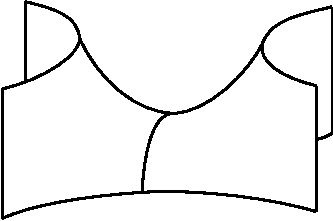
\includegraphics{saddle}
\caption{This is a saddle.}\label{fig:saddle}
\end{figure}

You can create tables like \cref{tab:sample}.

\begin{table}[ht]
\centering
\renewcommand{\arraystretch}{1.2} % Adds vertical padding
\begin{tabular}{>{\bfseries}l c r}
\toprule
Name & Value & Description \\
\midrule
Alpha & 1.23 & First entry \\
Beta & 4.56 & Second entry \\
Gamma & 7.89 & Third entry \\
\bottomrule
\end{tabular}
\caption{An example of a well-formatted table.}\label{tab:sample}
\end{table}



You can cite books, such as \emph{The \LaTeX\ Companion} by \textcite{GMS} or journal articles such as Franks and Richeson's ``Shift equivalence and the Conley index'' \parencite{FR}.

\printbibliography
\end{document}